\documentclass[]{article}
\usepackage{geometry}
\geometry{
	a4paper,
	total={170mm,257mm},
	left=0.75in,
	top=0.75in,
	right=0.75in,
	bottom=1in,
}
\usepackage{gensymb}
\usepackage{lipsum}
\usepackage{graphicx}
\usepackage{amsmath}
\usepackage{color}
\definecolor{MyBlue}{rgb}{0,0.3,0.6}
\usepackage[colorlinks=true,
            linkcolor=MyBlue,
            plainpages=false,
            citecolor=MyBlue,
            urlcolor=MyBlue]{hyperref}
\usepackage[url=true,
backend=bibtex,
style=authoryear-comp,
doi=true,
isbn=true,
backref=false,
dashed=false,
maxcitenames=2,
maxbibnames=99,
natbib=true]{biblatex}
\addbibresource{refrence.bib}
%opening
\title{\textbf{Surface waves in a Bingham fluid medium}}
\author{V. Sanjay, M. Jalal}
\date{}
\begin{document}
\maketitle
We study surface waves in a Viscoplastic medium using the Generalized Newtonian Fluid model for treating viscous forces.
\begin{figure}[h]
\begin{center}
 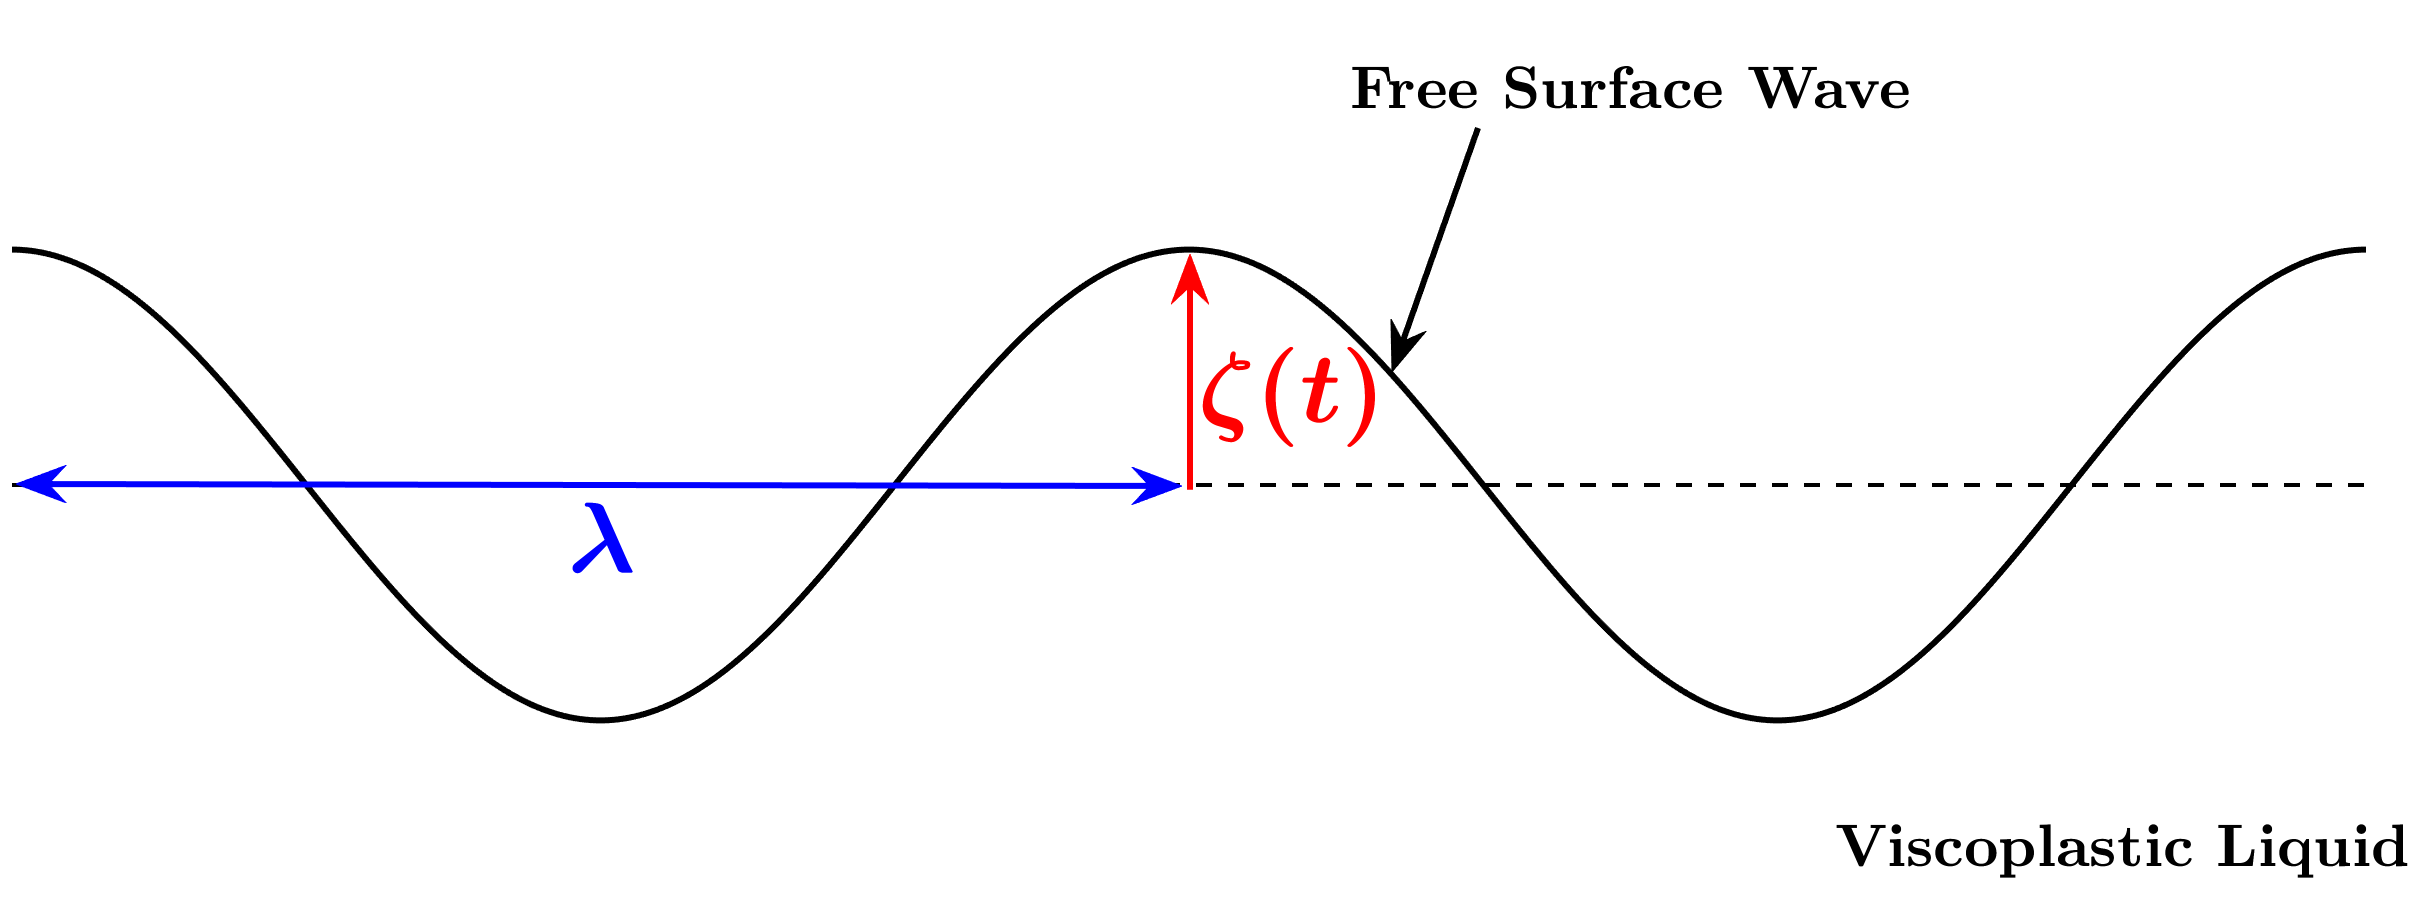
\includegraphics[width=0.75\textwidth]{Schematic}
 \caption{Schematic of the problem: Free Surface Wave in a Viscoplastic Fluid.
 We track the temporal variation of the amplitude of these oscillations $\left(\zeta\right)$.}
 \label{Figure::Schematic}
\end{center}
\end{figure}

\section{Regularization method for Non-Newtonian Fluids}\label{Section::Regularization}
In this section, we briefly describe the regularization method that we have implemented in \href{http://basilisk.fr/}{Basilisk}:\\
We first calculate the second invariant of the deformation tensor $\left(D_{ij} = 0.5\left(\partial_iU_j + \partial_jU_i\right)\right)$.
$$D_{11} = \frac{\partial u}{\partial x}$$
$$D_{12} = \frac{1}{2}\left( \frac{\partial u}{\partial y}+ \frac{\partial v}{\partial x}\right)$$
$$D_{21} = \frac{1}{2}\left( \frac{\partial u}{\partial y}+ \frac{\partial v}{\partial x}\right)$$
$$D_{22} = \frac{\partial v}{\partial y}$$
The second invariant is $D_2=\sqrt{D_{ij}D_{ij}}$ (this is the Frobenius norm)
$$D_2^2= D_{ij}D_{ij}= D_{11}D_{11} + D_{12}D_{21} + D_{21}D_{12} + D_{22}D_{22}$$
The equivalent viscosity is
$$\mu_{eq}= \mu_0\left(\frac{D_2}{\sqrt{2}}\right)^{N-1} + \frac{\tau_y}{\sqrt{2} D_2 }$$
\textbf{Note}: $\|D\| = D_2/\sqrt{2}$.\\
For Bingham Fluid, N = 1:
$$\mu_{eq}= \mu_0 + \frac{\tau_y}{\sqrt{2} D_2 }$$
Finally, $\mu$ is the minimum of of $\mu_{eq}$ and a large $\mu_{max}$. The fluid flows always, it is not a solid, but a very viscous fluid.
$$ \mu = min\left(\mu_{eq}, \mu_{max}\right) $$

\section{Numerical Simulations}
We solve the equations above along with the continuity equation $\left(\partial_{i}U_i = 0\right)$ and the full Navier-Stokes equation.
\begin{equation}
\hat{\rho}\left(\frac{\partial U_i}{\partial t} + \frac{\partial\left(U_iU_j\right)}{\partial X_j}\right) = -\frac{\partial P}{\partial X_i} + Oh\frac{\partial}{\partial X_j}\left(\hat{\mu}_{eq}D_{ij}\right) + \delta_s\hat{n}_i
\end{equation}
Symbols have their usual meaning. The Ohnesorge number is defined as $\left(Oh = \mu_0/\sqrt{\sigma\rho\lambda}\right)$. Here, $\lambda$ is the wavelength of the initialized standing surface wave, such that the amplitude of oscillation for the surface wave is given by:
\begin{equation}
a(x,t) = \zeta(t)cos\left(2\pi\frac{x}{\lambda}\right)
\end{equation}
We use Volume of Fluid (VOF) and height function \citep{popinet2009accurate} for interface reconstruction. The code used for the present study can be found at \href{http://basilisk.fr/sandbox/vatsal/GenaralizedNewtonian/SurfaceWavesBingham.c}{\cite{vatsal}}. Figure~\ref{Figure::Results} represents the variation of the amplitude of surface wave oscillation over time.
\begin{figure}
\begin{center}
 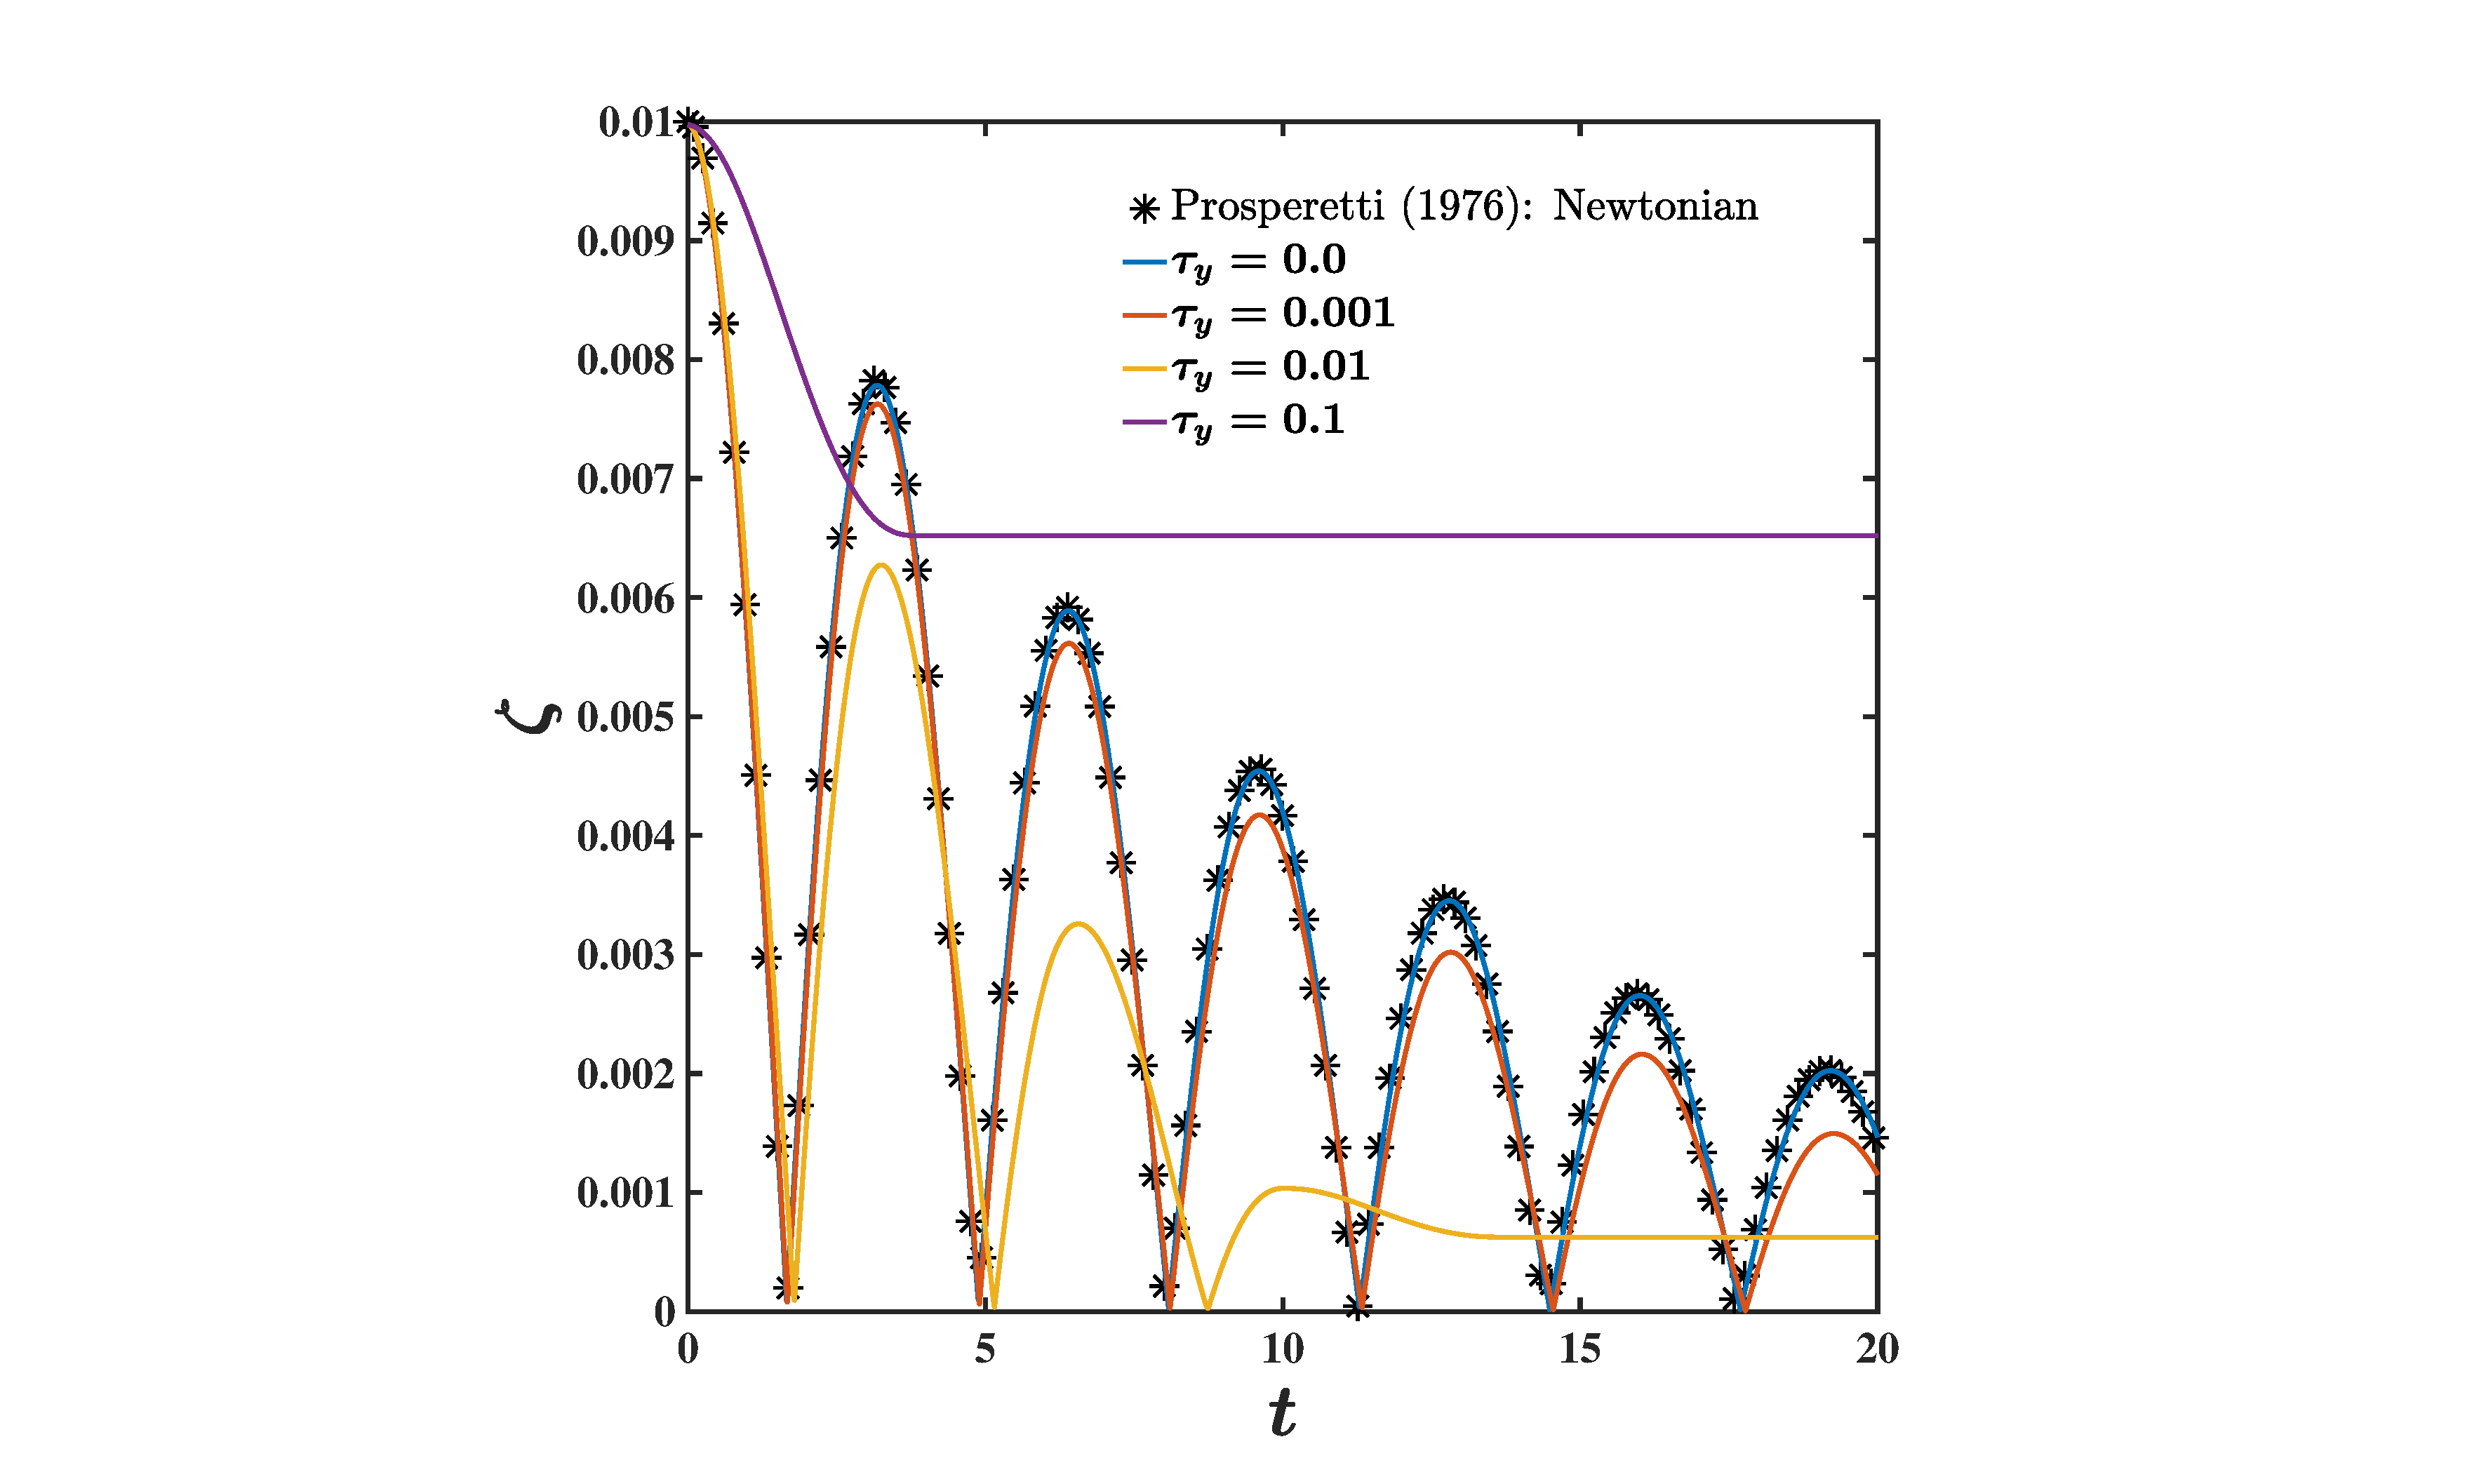
\includegraphics[width=\textwidth]{Amplitude}
 \caption{Variation of the amplitude of oscillations with time. Initially, all fluids yield because of the high-stress initial condition. In time, oscillation is arrested as the fluid reaches the plastic limit. This stopping time decreases with increasing yield stress $\tau_y$.}
 \label{Figure::Results}
\end{center}
\end{figure}
\section{Theory}
\subsection{Newtonian Case}
Following \cite{prosperetti1976viscous}, the equation of motion for the interface can be written as:
\begin{equation}
\frac{\partial^2 \zeta}{\partial t^2} + 4\epsilon\frac{\partial \zeta}{\partial t} + \zeta - 4\epsilon^2\int_0^t\left\{\frac{e^{-\epsilon(t-\theta)}}{\sqrt{\pi\epsilon(t-\theta)}} - erfc\left(\sqrt{\epsilon(t-\theta)}\right)\right\}\frac{d}{dt}\left(\zeta(\theta)\right)d\theta = 0
\end{equation}
The above equation is a simplified form of the equation presented in \cite{prosperetti1981motion}, under the assumption: $\rho_{\mbox{upper}} \to 0\:\&\:\rho_{\mbox{lower}} = \rho, \nu_{\mbox{lower}} = \nu$ and can be solved using Laplace Transformation. If $\hat{\zeta}(s)$ is the Laplace Transformation of $\zeta(t)$, then the solution of the above equation in the Laplace Space with $\zeta(0) = 1.0$ and $\dot{\zeta}(0) = 0.0$ is:
\begin{equation}
\hat{\zeta}(s) = \frac{1}{s}\left(1 - \frac{1}{1 + s^2 + 4\epsilon s + 4\epsilon^2 - 4\epsilon\sqrt{\left(1+s/\epsilon\right)}}\right)
\end{equation}
Here, $\omega^2 = gk + \frac{\sigma}{\rho}k^3$ and $\epsilon = \frac{\nu k^2}{\omega}$. The above equation can be inverted using the MATLAB code by \cite{MATLAB} which is based on the numerical method described by \cite{abate2006unified}.
\subsection{Non-Newtonian Case}
We are still working on this. It would be interesting to study the surface waves in Viscoplastic medium theoretically. Notably, we are looking for a method to get the stopping time of these waves as a function of the Yield Stress. For now, we only have the numerical simulations.
\printbibliography
\end{document}
